% This must be in the first 5 lines to tell arXiv to use pdfLaTeX, which is strongly recommended.
\pdfoutput=1
% In particular, the hyperref package requires pdfLaTeX in order to break URLs across lines.

\documentclass[11pt]{article}

% Remove the "review" option to generate the final version.
\usepackage{acl}

% Standard package includes
\usepackage{times}
\usepackage{latexsym}
%\usepackage[normalem]{ulem}  % For strikethrough
% \usepackage{booktabs} % for better table rules
% \usepackage{array}    % for advanced tabular formatt
% For proper rendering and hyphenation of words containing Latin characters (including in bib files)
\usepackage[T1]{fontenc}
\usepackage{listings}
% For Vietnamese characters
% \usepackage[T5]{fontenc}
% See https://www.latex-project.org/help/documentation/encguide.pdf for other character sets

% This assumes your files are encoded as UTF8
\usepackage[utf8]{inputenc}
\usepackage[inline]{enumitem}
\usepackage{tcolorbox} % For custom boxes
\usepackage[normalem]{ulem}

% This is not strictly necessary, and may be commented out.
% However, it will improve the layout of the manuscript,
% and will typically save some space.
\usepackage{microtype}

% This is also not strictly necessary, and may be commented out.
% However, it will improve the aesthetics of text in
% the typewriter font.
\usepackage{inconsolata}
\usepackage{amsmath}
\usepackage{booktabs}
\usepackage{multirow}
\usepackage{graphicx}

% If the title and author information does not fit in the area allocated, uncomment the following
%
%\setlength\titlebox{<dim>}
%
% and set <dim> to something 5cm or larger.

% \title{Towards Named Entity Recognition \& Entity Linking on Car Advertisements}

\title{%
    Shifting NER into High Gear: The Auto-AdvER Approach   %\; 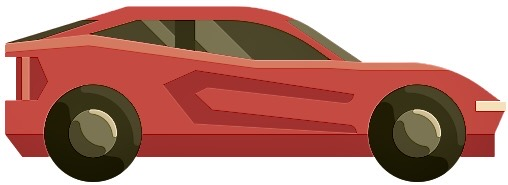
\includegraphics[scale=0.08]{figures/sport-car.jpeg}
}

% Possible titles:
% Towards Auto-AdvER: Automobile Advertisements NER Schema

% Gearing Up for Precision: Auto-AdvER's NER Schema in Automotive Advertising


% Accelerating NER in Automotive Ads with Auto-AdvER

% Navigating the Road of Automobile Ads: Auto-AdvER's NER Schema

% Shifting NER into High Gear: The Auto-AdvER Approach

% Author information can be set in various styles:
% For several authors from the same institution:
% \author{Author 1 \and ... \and Author n \\
        % Address line \\ ... \\ Address line}
% if the names do not fit well on one line use
        % Author 1 \\ {\bf Author 2} \\ ... \\ {\bf Author n} \\
% For authors from different institutions:
% \author{Author 1, Author 2 \\ Address line \\  ... \\ Address line
%         \And  ... \And
%         Author n \\ Address line \\ ... \\ Address line}
% To start a seperate ``row'' of authors use \AND, as in
% \author{Author 1 \\ Address line \\  ... \\ Address line
%         \AND
%         Author 2 \\ Address line \\ ... \\ Address line \And
%         Author 3 \\ Address line \\ ... \\ Address line}

% \author{First Author \\
%   Filippos Ventirozos \\
%   Affiliation / Address line 2 \\
%   Affiliation / Address line 3 \\
%   \texttt{F.Ventirozos@mmu.ac.uk} \\\And
%   Second Author \\
%   Affiliation / Address line 1 \\
%   Affiliation / Address line 2 \\
%   Affiliation / Address line 3 \\
%   \texttt{email@domain} \\}


\author{
Filippos Ventirozos\textsuperscript{\dag},
Ioanna Nteka*,
Tania Nandy*,
Jozef Baca*,
Peter Appleby* \and
Matthew Shardlow\textsuperscript{\dag} \\
\textsuperscript{\dag}\,Manchester Metropolitan University, John Dalton tower, Chester St, Manchester M1 5GD, UK \\
*\,Auto Trader UK, 1 Tony Wilson Place, Manchester M15 4FN, UK \\
\texttt{\{f.ventirozos, m.shardlow\}@mmu.ac.uk} \\
% \texttt{\{ioanna.nteka, tania.nandy, jozef.baca, peter.appleby\}@autotrader.com}
}



\begin{document}
\maketitle
\begin{abstract}

This paper presents a case study on the development of Auto-AdvER, a specialised named entity recognition schema and dataset for text in the car advertisement genre. Developed with industry needs in mind, Auto-AdvER is designed to enhance text mining analytics in this domain and contributes a linguistically unique NER dataset\footnote{The dataset will be made available upon publication.}. We present a schema consisting of three labels: `Condition', `Historic' and `Sales Options'. We outline the guiding principles for annotation, describe the methodology for schema development, and show the results of an annotation study demonstrating inter-annotator agreement of 92\% F1-Score. Furthermore, we compare the performance by using encoder-only models: BERT, DeBERTaV3 and decoder-only open and closed source Large Language Models (LLMs): Llama, Qwen, GPT-4 and Gemini. 
Our results show that the class of LLMs outperforms the smaller encoder-only models. However, the LLMs are costly and far from perfect for this task.
We present this work as a stepping stone toward more fine-grained analysis and discuss Auto-AdvER's potential impact on advertisement analytics and customer insights, including applications such as the analysis of market dynamics and data-driven predictive maintenance. Our schema, as well as our associated findings, are suitable for both private and public entities considering named entity recognition in the automotive domain, or other specialist domains.

\end{abstract}
% \footnote{The code used to run our experiments and associated necessary supplementary materials will be made available upon publication.}

\section{Introduction}
The automotive industry relies heavily on accurate data regarding vehicles that are manufactured, sold and resold. In particular digital businesses rely on information extracted from online sources, such as car advertisements, for various applications including market analysis, competitive intelligence and customer insights. Named entity recognition (NER) serves as a pivotal technique to transform unstructured text into structured data \cite{li2020survey}. However, the unique nature of car advertisements necessitates a specialised NER label schema. This paper introduces a novel automobile advertisements NER schema developed within an industry context, named Auto-AdvER (\textbf{Auto}mobile \textbf{Adv}ertisment \textbf{E}ntity \textbf{R}ecognition). 

In the present study, we introduce the guiding principles for forming the annotation labels and labelling their respective spans from text. This work introduces a novel framework for labelling car advertisements with key information. We anticipate the development of future schema which extend ours in subsequent research. With this schema, we hope to set a standard for text annotation studies within the automotive industry and beyond, demonstrating best practices for future development. By sharing our schema and data we also hope to encourage collaborative annotations from other interested parties from academia and industry. Specifically, our contributions lie in demonstrating:
\begin{enumerate*}
% \setlength{\itemsep}{-0.2em}
    % \item methodology for forming the schema
    \item A novel domain NER dataset
    \item The comparison of several applied NER models
    \item Critical discussion of these results, and applicability to the automotive industry and beyond.
\end{enumerate*}

% The remainder of the paper is structured as follows: In Section~\ref{sec:rel-work}, we introduce the NER task and NER studies in the automotive domain. Following this, in Section~\ref{sec:ner-schema}, we present our guidelines, the methodology for crafting them, and our resulting named entity tags (labels). In Section~\ref{sec:prel}, we document the annotation interface, metrics, and our preliminary results. Lastly, in Section~\ref{sec:discussion}, we discuss the results, mention future studies, and the applicability of the proposed NER schema in the wider industry. The full annotation schema including guidelines and a limited sample of annotations will be released upon publication of this work.

% The paper is organised as follows: Section~\ref{sec:rel-work} introduces the NER task and related studies. In Section~\ref{sec:ner-schema}, we describe our annotation process—including guidelines, methodology for crafting them, the annotation interface, and our resulting named entity labels. After discussing data attributes in Section~\ref{sec:data_attrs}, we present our experiments and inter-annotator agreement in Section~\ref{sec:exp}. This is followed by a discussion on wider applicability and future work in Section~\ref{sec:discussion}, and we conclude in Section~\ref{sec:concl}.

The paper is structured as follows: Section~\ref{sec:rel-work} introduces related NER studies in the automotive domain. In Section~\ref{sec:ner-schema}, we describe our annotation guidelines and methodology, and in Section~\ref{sec:data_attrs} we present the data properties and language. Section~\ref{sec:exp} presents our experiments and inter-annotator agreement (IAA) results. We discuss wider applicability and future work in Section~\ref{sec:discussion}, and conclude in Section~\ref{sec:concl}.

\section{Related Work}
\label{sec:rel-work}

% NER is an historic NLP task with early datasets formed for the CoNLL evaluation campaigns \cite{tjong-kim-sang-de-meulder-2003-introduction} focussing on general domain newstext. NER annotations typically use a BIO annotation schema with token-level tags indicating the token is at the \textbf{B}eginning, \textbf{I}nside or \textbf{O}utside of an NE. Later datasets focussed on linguistic annotation of large general domain corpora such as Ontonotes \cite{pradhan-etal-2013-towards}. 

% NER is a sequence labelling task. One can think it as a two step process. First, one needs to find from a text the spans applicable for labelling. Secondly, the identified spans are classified to a predefined class. Nonetheless, it is common in the literature to perform this task end-to-end \citep{JEHANGIR2023100017}. Typical approaches to NER consider a sequence labelling approach using BiLSTMs \cite{chiu-nichols-2016-named} or transformers \cite{hanh-2021-named}.

NER is a foundational sequence labelling task in NLP, with early datasets developed for the CoNLL evaluation campaigns \cite{tjong-kim-sang-de-meulder-2003-introduction} focusing on general news text. It involves identifying spans in text applicable for labelling and classifying them into predefined categories --- a process often performed end-to-end \citep{JEHANGIR2023100017}. Typical NER approaches have employed sequence labelling models such as conditional random fields \citep{keraghel2024recentadvancesnamedentity}, BiLSTMs \cite{chiu-nichols-2016-named} or transformers \cite{hanh-2021-named}.

% \subsection{NER in Specific Domains}

NER has been explored in various domains. Its applicability is useful for different domains and industries and acts typically as the first step towards information extraction projects. NER has been applied from biomedical applications \citep{fu-etal-2023-biomedical}, agriculture \citep{G2023120440} to music \citep{epure-hennequin-2023-human}. In these cases it is important to develop a bespoke annotation schema for the domain to represent the entities therein. 

% \subsection{NER in the Automotive domain}
% From what we know most studies currently tasks focus on speech conversation within cars but also

To the best of our knowledge, the only study addressing NER in the automotive domain is that of \citet{10499162}, who conducted NER on car accessories in Chinese. In contrast, our study investigates a more general set of named entities in car advertisements and is conducted in English.


\section{Dataset Overview}
\label{sec:ner-schema}
\subsection{Annotation Methodology}

To the best of our knowledge, this is the first schema for labelling car text advertisements. Consequently, we devised our own labels through the use of the action research framework \citep{Molineux2018UsingAR}. This work represents an effective collaboration between industry and academic partners, embedding NLP research into practice. 

% Our partnership aimed to understand the specific requirements of the project and deliver practical NLP solutions to enhance business processes and to facilitate the creation of new products.

Through our collaboration, we engaged extensively with industry data and resources and consulted with industry infrastructure engineers to leverage an in-depth understanding of the automotive domain. This in-house expertise was pivotal in crafting the initial set of labels and guidelines and to the success of our project, leading to the following core principles as outlined below.

\subsubsection{Core Principles}
\begin{enumerate}
\itemsep0em
 \item To extract the named entities schema, we initially employed coarser NER labels, with the intention of refining these entities through a subsequent step of entity linking. 

 % \item Our methodology included extracting only information that adds monetary value and provides a competitive advantage over other advertisements, based on the annotator's judgement.

 \item Each label was designed to be easily identifiable, typically answerable with a single question.

 \item  The aim was to annotate only factual statements, not opinions or personal sentiments. 
 
 % For instance, the statement ``low mileage'' is an opinion provided by the seller based on their judgement of the vehicle's age, and thus, it was omitted from annotation.

 % \item  Finally, similar to other NER studies, we aimed for each class to be semantically coherent to facilitate accurate predictions.
   
\end{enumerate}

% On the foundation of our annotation rules is to label spans which:
% \begin{enumerate}
%     \item are factual, not opinions. For instance, the statement ``low mileage'' is an opinion provided by the seller relative on their judgement of the age of the vehicle, hence, it would be omited from annotation.
%     \item add value to the ad, omit annotating standard or common sense things such as common opening hours, or references to mileage mentioning that now may be more, after the ad publication date.
% \end{enumerate}

% For more detail please visit \url{github} for the annotation guidelines.

\subsubsection{Iterations}
Our methodology for crafting the guidelines was inspired by the DevOps approach, as outlined in \citet{10.1145/2962695.2962707}. In DevOps two teams (Dev and Ops) collaborate through iterations of design and development compromising appropriately on design decisions to maximise efficiency. Initially the university-based \textbf{dev}elopment team created the classes and annotation guidelines. These were then discussed with the industry-based \textbf{op}eration\textbf{s} team comprised of domain-expert data scientists. The team had two members from the university partner (Dev) and three from the industry partner (Ops).

\paragraph{Initial Iterations}

During the first set of iterations, the development team proposed a draft of the guidelines. These proposals were then refined by the operations team, focusing on two main aspects: 
\begin{enumerate}
\itemsep0em
    \item The inclusivity of each class and the extent to which they covered various aspects of the advertisements.
    \item The identification of any omitted classes, which could either be sourced from other data or deemed non-essential.
\end{enumerate}

\noindent
% Following these discussions, the development team further defined the classes. In cases where a class lacked clarity regarding its encompassed aspects, the development team employed GPT-4 \citep{openai2024gpt4} to evaluate the semantic coherence of each aspect within the proposed class given its definition. The utilisation of large language models (LLMs) facilitated rapid prototyping, enabling the team to explore alternative classes and assess their detectability.

Following these discussions, the development team further refined the classes. When a class lacked clarity regarding its encompassed aspects, the team evaluated the semantic coherence of each aspect within the proposed definitions. Rapid prototyping enabled them to explore alternative classes and assess their detectability.

\paragraph{Secondary Iterations}

As the labels began to take shape, we entered the second set of iterations. Here, the development team introduced annotation tasks for the operations team. After the operations team completed these tasks, their feedback was discussed to further refine the guidelines. This feedback included analysis of challenging cases and observations on whether additional aspects should be incorporated.


\subsection{Named Entity Tags}

% To the best of our knowledge, this is the first English corpus on car text advertisements. Consequently, we devised our own labels. Our ongoing action research \citep{} collaboration with Auto Trader UK was instrumental in this process. This collaboration aimed to understand their requirements and deliver practical NLP solutions to enhance their processes or enable the creation of new products. We engaged with their data resources and consulted with infrastructure engineers to gain an in-depth understanding of the automotive domain, which was pivotal in crafting these labels. Additionally, we held meetings with the data scientists working with advertisements and NLP to discuss potential NER labels, ensuring they were semantically distinct, coherent, and capable of adding monetary value to advertisements.

% We then conducted a pilot test and refined the labels and their respective guidelines after annotating a sample of 80 advertisements—40 from traders and 40 from individual datasets—ourselves, covering a range of advert descriptions from shorter to longer texts.
% Following this process, we ended up with four named entity tags (also referred to as classes) for our study. We aimed for tags designed for an abstract type classification, to capture a broader portion of the text with a relatively small number of labels. These labels can then be subdivided into more specific subcategories, facilitating further NLP analysis of the sequences if needed. Specifically, we have identified four tags/classes:


% Following a thorough pilot test, where we annotated a sample of 80 advertisements—40 from traders and 40 from individual datasets—we refined the labels and their respective guidelines. This sample covered a range of advert descriptions, from shorter to longer texts, ensuring comprehensive coverage.

As a result of this process, we developed three named entity tags (these may also be referred to as `classes' or `labels') for our study. These tags were designed to classify text abstractly, capturing a broader portion of the content with a relatively small number of labels; thereby unlocking the potential for downstream application of entity linking. Specifically, we identified three tags:

% This approach allows for further subdivision into more specific subcategories, facilitating deeper NLP analysis of the sequences.

% There were three drivers that helped us refine these labels.
% We are in an ongoing process of action research \citep{} with Auto Trader UK to be able to understand their needs and provide practical NLP solutions that they can integrate and optimise their processes or create new products. During our period of active research we have played with multipe data resources and understand the automotive domain. Moreover, we have had meetings specifically rectifying the suggested NER labels in terms of whether they are semantically distinct, coherent, and can potentially add monetary value to the advertisement. 


% Firstly, from a qualitative approach, we conducted meetings with the Auto Trader's data scientists that do NLP, and discussed which labels are semantically distinct, coherent, and can potentially add monetary value to the advertisement. 

% Secondly, we carried out a topic modelling project using the Gemini model \citep{geminiteam2024gemini} and identified that most of the topics extracted belong to one of those labels. We detail later the parts that are not included in our annotation schema. 

% Thirdly, we refined the labels and their respective guidelines after annotating a sample of 80 advertisements—40 from traders and 40 from individual datasets—ourselves, ranging from shorter to longer advert descriptions. Specifically, we have identified four tags/classes:

\begin{itemize}[leftmargin=*,itemsep=0pt,parsep=0.2pt]
    % \item \underline{Feature Tag:} refers to the features of a car. A feature may be standard --- it comes included with the original purchase of the car. It may be optional, the person who procured the car from the manufacturer opted for additional features. The distinction between standard and optional features, is not straightforward, since, various retailers use their own terminology, manufacturers may have decided to move a feature from standard to optional or vice-versa influenced by market dynamics, and the accurate time of a car being manufactured for most advertisements is not undisclosed, making it challenging to trace the available standard and optional features of a specific car. The annotation would typically involve a noun or a noun and some adjective (e.g., ``heated seats'').
    \item \underline{Condition Tag:} which refers to the current condition of the vehicle in any positive, neutral or negative state. Instances of this may include engine noise, presence of scratches, tyre condition. The span would typically include a noun and an attribute (e.g., ``tyre tread is low''). 
    
    \item \underline{Historic Tag:} refers to an event that has happened to the car before the posting of the ad. Instances of those include past accidents, number of previous owners (e.g., ``2 owners''), component change and servicing (e.g., ``new cambelt fitted last august''). 

    \item \underline{Sales Options Tag:} refers to any tangible or service offered during the sale --- apart from the car. These could refer to part exchange offers, delivery, warranties and test drive. We developed a consesus through the DevOps methodology outlined above which led us to label only the noun with any adjectives and ignore any conditions. e.g., in the following sentence: \textit{\textbf{2 year warranty} when financed with Volvo Services, Terms and Conditions apply}, only the bold part would be annotated, but not either of the additional clauses.
    
\end{itemize}

%To some extent some of the above information can be derived from other resources. For instance, databases of vehicles do register MoT due, features, previous owner. Nonetheless, it's important to track this information since there could be a mismatch between the seller's information with the relevant databases.



\noindent

In Appendix~\ref{sec:appendix:labels} we disclosed part of the annotations guidelines which provide the definitions of each label and the detected sub-entities. Furthermore, additional entities encountered during our annotation phase were excluded from the study for reasons detailed in the appendix (see Appendix~\ref{sec:appendix:not_tracked} for documentation).


\label{sec:prel}
\subsection{Dataset Origin}

We used in-house data, based on a large proprietary database of current car advertisements. Half of the texts of these advertisements are written by customers, covering \textit{traders}, which are car dealerships with a large available stock of vehicles and high turnover and the other half by \textit{individuals} typically infrequently listing a single vehicle. 

% As such, each advertisement text contains a heterogeneous variety of unstructured information which is relevant to selling the vehicle, making these adverts a perfect case for NER. 




In addition, to ensure a representative sample for the trader dataset, we sorted traders by the number of their listings and selected those with the highest number of listings, as they typically follow a template for their sale ads. This approach ensured that we included template-based advertisements from traders. For the private dataset, we stratified the listings by UK region (e.g., "North West") and sampled a proportional number of car listings from each region. This method ensured that different regional variations of the English language are represented in our dataset.

An example of a (short) advert is given within the annotation interface presented in Figure \ref{fig:prodigy}.

% Auto Trader UK hosts a massive amount of vehicle listings every day. In our  study, we considered a snapshot of a one day in May 2024. From that snapshot we considered only the car listings, which amount the majority of the listings, and disregarded advertisements listed on Auto Trader's auction site. We retained only the advertisements aimed for retail selling.

% Following, our mission  was to retrieve a representative sample of car text advertisements. Upon being consulted from Auto Trader's domain expert data scientists we derived the following sampling process. We divided 100,000 car adverts into two groups, one comprising private ads\textemdash advertisements uploaded by individuals who want to sell their car\textemdash and the trader ads, creating two datasets of 50,000 each. This approach allowed us to compare the performance of our NER model on franchised (i.e. trader) text descriptions against those from individuals. Since it is mentioned that traders especially the larger ones tend to follow their own narrative or follow their own template, whereas advertisements from individuals would tend to vary significantly between them.





\subsection{Annotation GUI}

For our annotations we used Prodigy by spaCy \citep{prodigy}. We implemented a customised NER version which let our annotators choose amongst the three labels. Also, below the annotation text the interface would show the specifications of the vehicle that is being annotated for context. Figure \ref{fig:prodigy} shows an example of an annotated text.
\begin{figure}[ht]
    \centering
    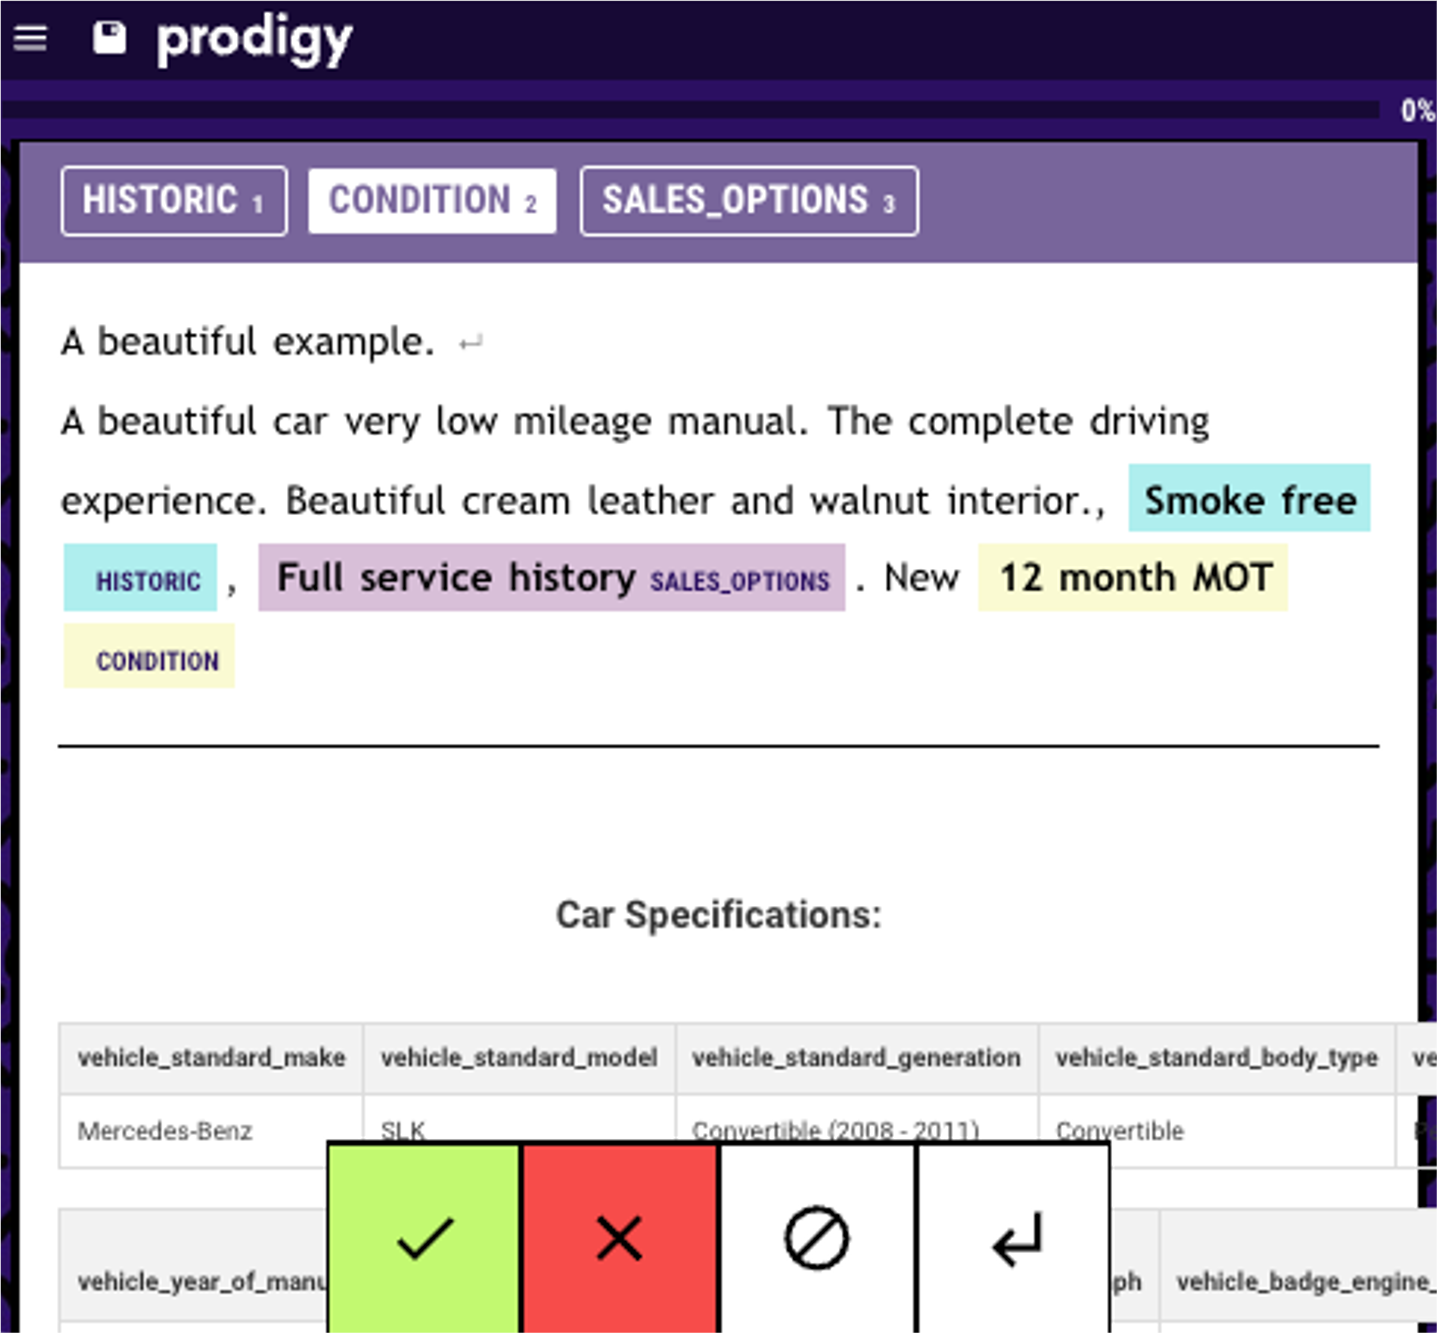
\includegraphics[width=\columnwidth]{figures/prodigy.png}
    \caption{An example of the annotation interface. It is a customised NER annotation using Prodigy.}
    \label{fig:prodigy}
\end{figure}

\subsection{Dataset Overview}
\label{sec:data_attrs}
% \subsubsection{Dataset Statistics}

In our dataset, we analysed a total of 605 advertisements, amounting to 104,382 tokens. Notably, 30 of these advertisements (approximately 5\%) contained no identifiable entities. These ads typically consisted solely of sales pitches, car standard/optional features, or were very short (e.g., ``2.0-liter engine BMW'') without further descriptive or contextual information. In Table~\ref{tab:stats}, we present the total number of labels and tokens for each label in our dataset.

\begin{table}[t]
\centering

\resizebox{\columnwidth}{!}{%
\begin{tabular}{llll}
\hline
Number of & CONDITION & HISTORIC & \begin{tabular}[c]{@{}l@{}}SALES\\ OPTIONS\end{tabular} \\ \hline
\# Labels & 573       & 794      & 2,134                                                  \\
\# Tokens & 13,107      & 21,227    & 38,358                                                  \\ \hline
\end{tabular}%
}
\caption{Distribution of labels and their corresponding tokens in our dataset.}
\label{tab:stats}
\end{table}

% \subsubsection{Linguistic Analysis}

Compared to other NER datasets from the literature our dataset would be most similar to ``noisy'' datasets such as WNUT16 \citep{strauss-etal-2016-results} and Twitter NER \citep{ritter-etal-2011-named}. The similarities lie in the use of colloquial language, typos, non-standard formatting, abbreviations, and some instances of emoticons. However, the unique aspect of our dataset is that it is designed for users to submit sales pitches for their cars. Consequently, distinct features include the use of telegraphic-style language, non-standard grammar (e.g., missing connecting words), the omission of contextual information and capitalisation to capture the buyer's attention. Additionally, we observed extensive use of persuasive language (e.g., positive adjectives), direct calls to action (e.g., imperative sentences encouraging viewers to call or not to miss out on the opportunity), and detailed lists of features, attributes or services.



Moreover, we noticed a clear divide between the texts from traders and individuals. Traders typically use a customisable template-based approach to ensure professionality and efficiency whereas the individual posts hugely vary in style and tone. Moreover, traders tend to list all \textit{Sales Options} that they offer.

% For our analysis we chose half of the instances to be from traders and half from individuals to reflect the full range of adverts available to us.


% \subsubsection{Labels}
In our linguistic observation of the tags, we found distinct linguistic features across different categories. The \textit{Condition} tag uses noun phrases and descriptive adjectives to provide detailed descriptions of the car’s current state, such as mileage, MOT status, and the condition of components. The \textit{Historic} tag predominantly employs past participles and passive constructions to reflect past actions taken on the vehicle, supplemented by temporal adverbials to mark the timing of these events, and noun phrases to detail ownership and maintenance history. Meanwhile, the \textit{Sales Options} tag features noun phrases to list services and offers.

% For the Condition tag, which reflects the current known facts about the car, we noticed that noun phrases and descriptive adjectives, as well as adjective phrases, modify nouns to provide detailed descriptions. These are used to highlight aspects such as mileage, MOT status, or the condition of components.

% For the "Historic" tag, we observed that past participles and passive constructions are common, reflecting actions that have been performed on the vehicle. Temporal adverbials (e.g., "2 months ago," "in 2021") are used to specify when events occurred. Additionally, noun phrases efficiently convey information about ownership and maintenance history.

% For the "Sales" tag, noun phrases (NPs) dominate, listing services and offers. Adjectives and modifiers are used extensively to enhance appeal, with terms like "personalized" and "low rate." Additionally, clauses may be employed to state availability or terms.

\section{Experiments}
\label{sec:exp}
\subsection{Evaluation Metric}
For evaluation we used an adjusted F1-score for NER. We report the partial match based on \citet{segura-bedmar-etal-2013-semeval} who take into consideration various categories of errors \citep{chinchor-sundheim-1993-muc}. Specifically, they report:
\begin{enumerate}
\itemsep0em
    \item $COR$rrect, when the NER spans between the gold standard and the prediction match entirely
    \item $INC$orrect, when the spans match, but the label is different
    \item $PAR$tial, when the spans overlap and have the same label
    \item $MIS$sing, when a gold annotation span is not predicted
    \item $SPU$rious, when a model predicts spans which do not exist in the gold standard.
\end{enumerate}
Following this, we define the possible and actual matches as follows:

% Possible (Number of gold-standard annotations contributing to the final score)
\begin{displaymath}
\begin{aligned}
POS\text{sible} &= COR + INC + PAR + MIS \\
&= TP + FN \\
ACT\text{ual} &= COR + INC + PAR + SPU \\
&= TP + FP
\end{aligned}
\end{displaymath}

% Precision are recall can be characterised as follows in the 
% \textbf{exact match} setting:
% % Exact Match (for both strict and exact scenarios)
% \begin{displaymath}
% \begin{aligned}
% \text{Precision} &= \frac{COR}{ACT} \\
% &= \frac{TP}{TP+FP}
% \end{aligned}
% \end{displaymath}

% \begin{displaymath}
% \begin{aligned}
% \text{Recall} &= \frac{COR}{POS} \\
% &= \frac{TP}{TP+FN}
% \end{aligned}
% \end{displaymath}

We make use of the partial match \citet{segura-bedmar-etal-2013-semeval}, the precision are recall can be characterised as follows:% Partial Match (for partial and type scenarios)
\begin{displaymath}
\begin{aligned}
\text{Precision} &= \frac{COR + 0.5 \times PAR}{ACT} \\
&= \frac{TP}{TP+FP}
\end{aligned}
\end{displaymath}

\begin{displaymath}
\begin{aligned}
\text{Recall} &= \frac{COR + 0.5 \times PAR}{POS} \\
&= \frac{TP}{TP+FN}
\end{aligned}
\end{displaymath}

\noindent
We utilise the F1-score (the harmonic mean between precision and recall) for IAA by applying it with one annotator serving as the gold standard against the other. Cohen's Kappa is widely recognised as the preferred metric for IAA, having been developed to address the shortcomings of percentage agreement by accounting for chance agreement, which percentage agreement (e.g., accuracy) does not \citep{McHugh2012}.  However, research in information extraction \citep{brandsen-etal-2020-creating, richie-etal-2022-inter} has pointed out its shortcomings. Specifically, in the context of NER, it is observed that this task involves tagging sequences of words, which do not correspond to the concept of true negatives present in typical classification tasks. These true negatives are necessary for calculating the Kappa statistic. As a result, these studies have determined that the F1-score is more suitable.


\subsection{Inter Annotator Agreement}

%At the moment of writing this paper we have some preliminary results with one annotator from the ops groups against one from the dev group, who have completed both annotation iterations. Overall, on 20 advertisements a symmetric average between the dev and ops is 72\% for the exact match and 80\% for the partial match. Overall, the results indicated around 6\% more precision than recall.

To demonstrate the use of our schema, we have double pass annotated 86 advertisements using one annotator from the development team and one annotator from the operations team. To calculate the agreement we consider the dev annotations as the gold standard and calculate precision and recall for the partial match setting as described above. This provides us a partial match F1-score of 92\%, precision being a bit higher, 93\%, than recall with 91\%. We have included the breakdown of the matches identified for each category between the two annotators in Table~\ref{tab:res_labels}. 

\begin{table}[h]
\centering
\resizebox{\columnwidth}{!}{%
\begin{tabular}{lccccc}
\toprule
\textbf{Label} & \textbf{COR} & \textbf{INC} & \textbf{PAR} & \textbf{MIS} & \textbf{SPU} \\
\midrule
CONDITION & 93\% & 2\% & 1\% & 2\% & 1\% \\
HISTORIC & 86\% & 3\% & 7\% & 3\% & 1\% \\
SALES\_ & \multirow{2}{*}{83\%} & \multirow{2}{*}{1\%} & \multirow{2}{*}{10\%} & \multirow{2}{*}{4\%} & \multirow{2}{*}{2\%} \\
OPTIONS &  &  &  &  &  \\
\bottomrule
\end{tabular}
}
\caption{Analysis of agreement for each annotation category on the 82 double-annotated documents.}
\label{tab:res_labels}
\vspace{-1.5em}
\end{table}


% We note that the \textit{Feature}, \textit{Condition} and \textit{Sales Option} categories all have an exact match percentage of 66-71\%, with this rising to 76-89\% when partial matches are also included. 
%The analysis indicate that there may still be some room for improvement since the Ops is conservative, they keep missing some labels. 
% Moreover, some labels which are HISTORIC are misinterpreted (INC) as another class, our analysis showed that this is most often CONDITION.



% Looking ahead, training more the Ops and emthe annotation guidelines and another set of iteration to show how to annotate would potentially yield better results.

\subsection{Models}
For our experiments, we utilised eight models. Firstly, given that our task was somewhat context-intensive, where depending on the context one might choose to highlight or ignore a span of tokens, we opted to use transformer-based models.

Firstly, we tested two type of encoder architecture transformers. One was BERT \citep{devlin-etal-2019-bert} (base and large)\footnote{\href{https://huggingface.co/google-bert/bert-base-cased}{bert-base-cased} \& \href{https://huggingface.co/google-bert/bert-large-cased}{bert-large-cased}}. The other was DeBERTaV3 \citep{he2021debertav3,he2021deberta} (base and large)\footnote{\href{https://huggingface.co/microsoft/deberta-v3-base}{deberta-v3-base} \& \href{https://huggingface.co/microsoft/deberta-v3-large}{deberta-v3-large}}. We trained them according to the token-classification\footnote{\href{https://github.com/huggingface/transformers/tree/main/examples/pytorch/token-classification}{token-classification}} methodology from HuggingFace \citep{wolf2020huggingfacestransformersstateoftheartnatural}. Since, our dataset was not particularly large, we used a lower learning rate than the default and a higher number of epochs; these can be found in Listing~\ref{lst:hyperparameters} in Appendix \ref{sec:hyper-params}.




% Initially, we tested BERT \citep{devlin-etal-2019-bert} large\footnote{\href{https://huggingface.co/google-bert/bert-large-cased}{bert-large-cased} \& \href{https://huggingface.co/google-bert/bert-base-cased}{bert-base-cased}} using the NER setting\footnote{\href{https://github.com/huggingface/transformers/tree/main/examples/pytorch/token-classification}{token-classification}} from HuggingFace \citep{wolf2020huggingfacestransformersstateoftheartnatural}. We adhered to the default hyper-parameters, with the slight adjustment of setting the batch size to 2 to accommodate the capabilities of an M1 Max CPU. We also set the number of epochs to be high, 20, and determined the best epoch to be used for prediction.

Secondly, we experimented with two open and two closed sourced decoder type, large language model, architectures. Specifically, these were: GPT-4o \citep{openai2024gpt4}, Gemini Flash \citep{geminiteam2024gemini}, Llama \citep{grattafiori2024llama3herdmodels} and Qwen \citep{yang2024qwen2technicalreport}. % \footnote{The gpt-4o-2024-11-20 version was used via the OpenAI API \href{https://platform.openai.com/}{platform.openai.com}.} \cite{openai2024gpt4} , 
    % using the OpenAI API\footnote{\href{https://platform.openai.com/}{platform.openai.com}} 
Their precise versions are in Listing~\ref{lst:llm_versions}.
For prediction with the LLMs we followed the NER setting as proposed by \citet{wang2023gptnernamedentityrecognition}
We employed 100 samples from the training data in an in-context learning (ICL) scenario. Specifically, for each label, to clarify for the LLM, we empirically added the label's definition at the beginning of the prompt and then used a chat alternating history to demonstrate how a text should be labelled. At the end of the prompt, we included a sample from the test data and collected the output. The output would replicate the input text, but a named entity would be marked by prefixing with `@@' and suffixing with `\#\#' to segment it from the rest of the text. An example is shown in Appendix~\ref{sec:appendix:prompt}. In cases where the text was not copied verbatim, we tackled this issue using an alignment library\footnote{\href{https://pypi.org/project/pytextspan/}{pytextspan}}.
% If two labels overlapped, we retained the one with the highest log probability, i.e., the model's perceived confidence. For our experiments we would use temperature zero, to target the high probability tokens.

All training and inference for the open-source models were performed on NVIDIA H100 Hopper graphics cards.

\subsection{Results}
For our experiments, we measure performance across three folds of the dataset, where the test sets were mutually exclusive. Each fold used 70\% of the instances for training, with 15\% each for validation and testing. The decoders would not require the validation dataset, since we did not fine-tune them. In some cases, the generations were incorrect and could not be recovered, even with our alignment library, this occurred rarely, less than 1\% in each fold. The overall results for each fold are presented in Table~\ref{tab:res}. 


\begin{table}[ht]
\small
\centering
% \setlength{\tabcolsep}{2pt} % Adjust the column separation here
%\resizebox{1.1\columnwidth}{!}{%


\begin{tabular}{cccc}
\hline
\textbf{Model}                                              & \textbf{Precision}                & \textbf{Recall}                   & \textbf{F1-score}                 \\ \hline
BERT-base                                                   & 28.7 $\pm$1.0 & 35.7 $\pm$1.3 & 32.0 $\pm$0.8 \\
BERT-large                                                  & 29.3 $\pm$1.3 & 36.7 $\pm$0.9 & 33.0 $\pm$0.8 \\
\begin{tabular}[c]{@{}c@{}}DeBERTaV3-\\ base\end{tabular}   & 34.0 $\pm$0.8 & 39.0 $\pm$0.8 & 36.3 $\pm$0.5 \\
\begin{tabular}[c]{@{}c@{}}DeBERTaV3-\\ large\end{tabular}  & 33.3 $\pm$1.3 & 39.3 $\pm$1.3 & 36.0 $\pm$0.8 \\ \hline
GPT-4o                                                      & 72.3 $\pm$1.9 & \textbf{54.7 $\pm$1.7} & \textbf{62.0 $\pm$0.8} \\
\begin{tabular}[c]{@{}c@{}}Gemini 1.5 \\ Flash\end{tabular} & 71.0 $\pm$1.6 & 50.0 $\pm$3.3 & 58.7 $\pm$2.1 \\
\begin{tabular}[c]{@{}c@{}}Llama 3.1 \\ 70B it\end{tabular} & 74.3 $\pm$1.7 & 44.7 $\pm$2.5 & 55.7 $\pm$2.5 \\
\begin{tabular}[c]{@{}c@{}}Qwen 2.5 \\ 72B it\end{tabular}  & \textbf{75.7 $\pm$2.9} & 35.0 $\pm$1.4 & 47.7 $\pm$1.9 \\ \hline
\end{tabular}
%}
\caption{The averaged and standard deviation precision, recall and F1 results in percentages across the three folds for each model. The "it" stands for instruction-tuned. The numbers in bold are the highest in their category.}
\label{tab:res}
\end{table}




% \begin{table}[ht]
% \centering
% \resizebox{0.95\columnwidth}{!}{%
% \begin{tabular}{ccccc}
% \hline
% \textbf{Model}        & \textbf{Fold} & \textbf{Precision} & \textbf{Recall} & \textbf{F1-score} \\ \hline
% \multirow{3}{*}{BERT} & 1             & 26\%               & 36\%             & 30\%               \\
%                       & 2             & 30\%                & 37\%             & 33\%               \\
%                       & 3             & 28\%                & 36\%             & 31\%               \\ \hline
% \multirow{3}{*}{GPT}  & 1             & 70\%                & 53\%             & 60\%               \\
%                       & 2             & 74\%                & 58\%             & 65\%               \\
%                       & 3             & 73\%                & 57\%             & 64\%               \\ \hline
% \end{tabular}
% }
% \caption{Evaluation results for BERT-large and GPT-4o across three folds.}
% \label{tab:res}
% \end{table}



% \begin{table}[h!]
% \centering

% \resizebox{\columnwidth}{!}{%
% \begin{tabular}{lccc}
% \toprule
% \textbf{Model and Label} & \textbf{Precision} & \textbf{Recall} & \textbf{F1-score} \\
% \midrule
% \multicolumn{4}{c}{\textbf{BERT-large Scores}} \\
% \midrule
% CONDITION         & 25\%  & 28\%  & 26\%  \\
% HISTORIC          & 31\%  & 45\%  & 36\%  \\
% SALES OPTIONS     & 27\%  & 35\%  & 30\%  \\
% \midrule
% \multicolumn{4}{c}{\textbf{GPT-4o Scores}} \\
% \midrule
% CONDITION         & 66\%  & 52\%  & 58\%  \\
% HISTORIC          & 68\%  & 53\%  & 60\%  \\
% SALES OPTIONS     & 76\%  & 58\%  & 66\%  \\
% \bottomrule
% \end{tabular}
% }
% \caption{Averaged performance metrics across the three folds for BERT-large and GPT-4o models.}
% \label{tab:label_metrics}
% \end{table}



\section{Discussion}
\label{sec:discussion}
Our effort represents the first annotation schema for car advertisements, which has been developed based on industry needs. 
%After iterations between the university and industry teams, we defined the initial entities. We evaluated the IAA score, achieving a promising F1 score of 92\%. 
One issue that emerged was that there were relatively more partial matches for the \textit{Sales Options} and \textit{Historic} labels (i.e., only segments of an entity are matched against the ground truth). Although we put effort into mitigating this issue by editing the annotation guidelines, we attribute it to the nature of the labelling. \textit{Historic} labels often refer to past events, leading annotators to include additional, possibly extraneous, contextual information. \textit{Sales Options} labels, owing to their liberal use of adjectives to describe services a dealer offers, create ambiguity about which aspects are sufficiently factual or necessary for inclusion.


For the NER prediction task, we tested eight models in a three-fold setting. The results, shown in Table \ref{tab:res}, indicate that the large decoder models have an advantage over the smaller encoder models. Notably, the precision is higher than the recall. This may be due to the fact that we utilised only 100 ICL examples per fold to maintain fairness in comparison between the models and to reduce computation time and cost. Possible improvements could include enlarging the context length, implementing boosting or voting among the LLM generations, or fine-tuning an LLM for this task.


% From the results, Table~\ref{tab:label_metrics}, of GPT-4o sales options has higher performance than the other lables. THis could be attributed to the disparity of the frequency of training data, Table~\ref{tab:stats}. Whereas in the IAA we noticed that the \textit{Condition} tend to have higher results. This shows room for improvement.

% It was omniprsecent, in IAA and in the models comparison, that the Sales Options and the Historic tend to have higher partial matches (i.e. only some part of an entity is matched against ground truth), due to the nature of the labelling, since the historic often refers to an event in the past, annotators taking the liberty to include additional contextual information, and the sales options make an extensive use of adjectives on the services a dealer advertises causing confusion on which are factual enough to include.

% On all the comparisons Somewhat the historic and the condition have higher percentages of missing and spurious, we believe it is because the judgement of something being a condition of a car or just a sales pitch (e.g., ``good tyres'', ``no accidents'', ``smoke free'').



% From the results presented in Table~\ref{tab:label_metrics}, it is evident that the GPT-4o model's performance on \textit{Sales options} is superior to that of other labels. This disparity could largely be attributed to the differing frequencies of training data, as shown in Table~\ref{tab:stats}. Contrastingly, in the IAA analysis, the \textit{Condition} label tends to yield higher accuracy. This discrepancy indicates potential areas for improvement.



% Across all comparisons, the labels for \textit{Historic} events and \textit{Condition} exhibit higher incidences of missing and spurious entries. We hypothesise that this occurs due to the difficulty in discerning whether certain descriptors pertain to the condition of a car or are merely part of a sales pitch—for example, phrases such as ``good looking tyres'', ``no accidents'', or ``smoke-free''.

% On general across the datasets the incorrect labels were low. 

% We will develop it more...

% FROM IAA
% We expect the reason lies in expressing the SALES OPTIONS products with more adjectives (``warranty'' as opposed to ``6-month warranty'' or ``service book'' as opposed to ``BMW full serviced history service book'').

% The decision lies many times in the perception of what is a service they offer on the basis if this is something advantageous over other car adverts (with a typical service) or not.
% The HISTORIC labelling is challenging since is about annotating an event.

% Typically, an event would have a trigger word and some lexical units, in our case we would label the whole span and leave the event extraction on a latter step. 

% The categories that we have proposed allow us to annotate entities which are factual and add value to an advertisement. 
%Our findings demonstrate that some labels are prone to have a different span, hence, opting for including partial match seems a more fair detection of the features. 
% We noted that although we were able to perform well in the strict setting of exact match, our performance in the partial match setting was much higher. 

% Further annotator training and refinement of the guidelines will allow us to improve the annotator agreement. We will also expand the annotator team and annotate a wider set of advertisements.
%Nonetheless, our error analysis indicate that our annotator tend to miss some labels, more training before the annotation or having an large language model hinting where they could annotate could ameliorate the issue.

% \paragraph{LLM Hinting}
% Looking forward we want to aid the annotator to annotate without leaving out spans. 

% \subsection{Named Entity Recognition}
%\paragraph{Contextual NER}
%It was evident to us that predicting the feature labels is dependent on the available features that the car's manufacturer offers. Hence, looking forward during our NER modelling we want to include the context of the available features for predicting the features mentioned in the text. 

% All in all, we belive we got encouraging results, but with still some room of imrpovement.

\paragraph{Next Steps}
We identified several types of entities emerging from our data. A non-exhaustive list of these entities is documented in Appendix~\ref{sec:appendix:labels}. Looking ahead, we aim to develop a taxonomy and undertake entity linking to associate the extracted named entities with their specific corresponding entities. \textbf{Entity linking} can facilitate a more in-depth analysis of car advertisements and enable \textbf{slot-filling} to derive the corresponding values of specific mentions.


\paragraph{Wider Applicability}
Exploring market dynamics through an NER schema reveals intricate insights into how subjective elements—such as the number of previous owners or a vehicle's maintenance history—are valued across different regions. These dynamics become even more pronounced when examining trends in \textit{Sales Options} like warranties, financing, and part-exchanges, which vary significantly depending on economic conditions and regional preferences. This raises questions about whether a robust economy alters these trends and what consumers fundamentally expect from their dealings with car dealerships. Additionally, the \textit{Condition} of vehicles—for instance, the presence of new tyres or the extent of scratches—plays a critical role in shaping consumer decisions.

The application of NER data extends to safety and accident analysis, where patterns categorised by location and severity provide essential insights for police, insurance companies, and urban planners considering road expansions. Safety further intersects with reliability, as the data highlight recurring issues or defects in car models over time, prompting manufacturers to address potentially faulty components. Moreover, an NER model could be applied to car forums to extract information on failing components.

This detailed dataset supports the development of tools to educate car owners about necessary or upcoming maintenance, potentially revolutionising consumer knowledge and empowerment. Establishing this NER framework as a new benchmark allows for advancements toward fairer advertising practices by quantifying and highlighting instances of under-reporting and suggesting policies that may require the disclosure of certain types of accidents to enhance consumer awareness. Such comprehensive use of data ensures a more transparent marketplace and significantly enhances consumer safety and satisfaction.

% Furthermore, by analysing which cars were subject to recalls and the specific issues addressed, this dataset aids in regulatory and compliance monitoring. It holds significant implications for trade policies as well; regions showing limitations in car conditions or options might benefit from economic boosts to enhance their automotive markets, while areas with a prevalence of fraudulent practices may require stricter oversight and consumer protection measures. 



% We believe the text mining applicability from the proposed NER schema can leverage various stakeholders in the vehicle trading industry and beyond. Starting from the trading industry the potential that the schema can offer are: accurate evaluations of vehicle features, auto-complete suggestions when writing an advert, automatic generation of advert text, and evaluation of the quality of an advertisement. 
% %In addition, more analytics would be useful to detect which appeal to consumers such as different types of sales options.
% Our schema could also benefit car manufacturers who want to track the condition of vehicles through mining advertisements, or detect which features are popular with consumers.

% \subsection{Evaluation}


% In the new global economy, the intersection of technology and commerce has profoundly reshaped consumer behaviour, particularly in sectors such as automotive retail. This sector is increasingly mediated through online platforms that host vast quantities of data. Notably, in the UK recently, consumer demand in the automotive industry has been increasing \cite{cardealermagazine2024}, and buying a new car has been at the forefront of financial life goals for many young adults in the \cite{gbnews2024}. This trend is fuelling digital platforms like Auto Trader UK, which features almost half a million vehicle listings each day—a rich dataset yet largely untapped by sophisticated analytical tools.

% Addressing this gap, our research employs natural language processing (NLP) to mine and interpret this extensive data reservoir. Specifically, we deploy named entity recognition (NER) to extract key information from car advertisements, focusing on optional features, vehicle condition, pricing strategies, and dealership details. Such targeted information extraction is critical for enhancing user engagement and improving market analyses. By integrating NLP into the automotive domain, this paper not only broadens the scope of computational linguistics but also contributes to smarter consumer tools and more nuanced industry insights...


%  Currently, a car advertisement is evaluated by the car's derivative\footnote{Loosely defined as the most fine-grained categorisation of a car. Considering the hierarchy brand > model > trim level > derivative.} similarity to other current or historic car advertisements and the amount of optional features they have. Current methodologies omit other parts of the advertisements. These include information about the condition of the car, components replaced in the car and sales options that may not be undisclosed in the advertisement fields.
% Todo: Write implications



% \section{Related Studies}





% \subsubsection{Silver Standard Annotation}
% Auto Trader UK utilises a bespoke rule-based algorithm to identify optional features in car advertisements, taking input from the free-text description section of an advertisement. Additionally, the Auto Trader website currently allows users to manually upload optional features one at a time and choose from a predefined list of possible options. However, our research concentrates on features that may not appear on the provided list, or those that users have opted to describe in the free-text section instead of selecting from the list. Consequently, we have utilised this algorithm to extract optional features from the free-text sections for our dataset.

% Following to construct our silver annotation dataset, we based our methodology on GPT-NER. However, we included domain knowledge from the known fields of each advert. We utilised in-context learning to use as examples in the prompt. The examples were drawn from text-ad samples that varied in text length and we made sure that half of the examples had optional features mentioned, since a lot of text ads were found to not include the optional features in the text description.




% \subsubsection{Gold Standard Annotation}



% \subsection{Dataset Statistics \& Splits}
% The amount of optional features extracted from Auto Trader's algorithm amounts to 26\% and 21\% for the individuals and the trader's respectively. However, is worth noting that trader's prefer listing the optional features on the Auto Trader's website dedicated section for listing them. This is evident in the dataset, since 40\% of optional features can be found from there compared with the mere 12\% from individuals. 

% We ensured our datasets were stratified across training, validation, and testing phases. In the end, based on this information, we stratified the two datasets into training, validation, and testing sets, allocating a 60\%, 20\% and 20\% to each respectively.




\section{Conclusion}
\label{sec:concl}
Our effort represents the first-ever English-language annotation schema and dataset for car advertisements. We collaboratively developed the entity annotation schema with involvement from industry and academia. The three labels we have chosen allow us to annotate entities that are meaningful, alter the value of the car, or affect the sale proposition. We achieved an encouraging IAA score and observed that LLMs surpassed the prediction accuracy of encoder models with GPT-4o leading in recall and f1-score, whereas Qwen in precision. Finally, we detailed how these labels can unlock future study of entity linking to obtain refined entities within each label, and discussed the wider applicability and contribution that stem from this work.

% Our effort represents the first-ever English language annotation schema and dataset for car advertisements. We collaboratively developed the entity annotation schema with involvement from industry and academia. The three labels we have chosen allow us to annotate entities that are meaningful, change the value of the car, the sale proposition. We got an encouraging IAA score and we observed that GPT-4o achieved comparable performance to that of IAA whereas BERT-large lacked, halfed of that of GPT-4o. Finally, we detailed how these labels can unlock future studies in entity linking to obtain refined entities in each label, and its wider applicability.


\section*{Limitations}
% We ascertained that most of the hyper-parameters of the BERT model remained unchanged; however, preliminary experimentation indicated, in some cases, only marginal improvements in performance outcomes.

Using closed-source LLMs complicates direct comparisons with open-source models due to their undisclosed training data. This lack of transparency can lead to data contamination issues in closed-source LLMs, obscuring true performance differences. Such factors make evaluations against open-source models incomplete and potentially misleading.

%One significant limitation of our current work is that it is still in progress, and the dataset used for our inter-annotator agreement analysis is relatively small. This limited dataset size may affect the generalisability of our findings and the robustness of our annotation schema. As a result, the reported inter-annotator agreement metrics might not fully capture the variability and complexity of car advertisements in a broader context. Future work will involve expanding the dataset to include a more diverse and comprehensive set of advertisements, which will allow for more thorough validation and potential refinement of our annotation schema.

% The dataset used for our inter-annotator agreement analysis is relatively small (20 instances). This may affect the generalisability of our findings and the robustness of our annotation schema. As a result, the reported inter-annotator agreement metrics might not fully capture the variability and complexity of car advertisements in a broader context. 

% Some of the identified information can be derived from other resources. For instance, databases of vehicles do register MoT information, car features or previous owner. Annotating this information manually allows us to track the accuracy of automated approaches based on databases and compare these to future proposed methods. There may also be mismatches between the seller's information and relevant databases which can be identified through techniques.


% ACL 2023 requires all submissions to have a section titled ``Limitations'', for discussing the limitations of the paper as a complement to the discussion of strengths in the main text. This section should occur after the conclusion, but before the references. It will not count towards the page limit.
% The discussion of limitations is mandatory. Papers without a limitation section will be desk-rejected without review.

% While we are open to different types of limitations, just mentioning that a set of results have been shown for English only probably does not reflect what we expect. 
% Mentioning that the method works mostly for languages with limited morphology, like English, is a much better alternative.
% In addition, limitations such as low scalability to long text, the requirement of large GPU resources, or other things that inspire crucial further investigation are welcome.

\section*{Ethics Statement}

In conducting this research, our primary motivation is to contribute to the greater good by enabling more informed consumers and enhancing the capabilities of individuals selling cars. We believe that a robust annotation schema for car advertisements will empower consumers with clearer, more reliable information and provide sellers with a tool to better present their products. Additionally, we acknowledge the ethical considerations associated with our work. We utilised LLMs. While this and similar models offer significant advancements, it is important to remain mindful of their substantial energy consumption and the environmental impact associated with their extensive use. Therefore, we advocate for a balanced approach, ensuring that the benefits of such technologies are weighed against their ecological footprint.


% Scientific work published at ACL 2023 must comply with the ACL Ethics Policy.\footnote{\url{https://www.aclweb.org/portal/content/acl-code-ethics}} We encourage all authors to include an explicit ethics statement on the broader impact of the work, or other ethical considerations after the conclusion but before the references. The ethics statement will not count toward the page limit (8 pages for long, 4 pages for short papers).

% \section*{Acknowledgements}
% AT employees and AT funding.

% Entries for the entire Anthology, followed by custom entries
\bibliography{output.bib}
% \bibliographystyle{acl_natbib}

\appendix

\section{Label's Definitions \& Identified sub-entities}
\label{sec:appendix:labels}

Below we specify our bespoke NEs for our own study applicable for Auto Trader's car advertisements.

\subsection*{Condition - Present Condition}
The \textit{Condition} category encompasses any valuable car-related information that is current as of the date the advertisement was posted online.
\begin{tcolorbox}[colback=gray!5!white, colframe=gray!75!black, title=Definition]
The \textit{CONDITION} label identifies any word or span of words in car advertisements that indicate the present material or documented condition of the vehicle, both positive and negative. This includes descriptions that reflect the car's current operational performance, mechanical state, aesthetic appearance, maintenance status, and legal classifications affecting its value or usability
\end{tcolorbox}
Specifically these include:
\begin{itemize}
    \item Tyre condition (i.e. trim level or mention of good condition)
    \item Interior condition (e.g., ``leather like new'')
    \item Exterior condition (e.g., ``presence of scratches'')
    \item Mechanical condition (e.g., ``engine noise'', ``gear not locking properly'')
    \item MoT due date or recent done MoT mentioned
    \item Service due date or recent done Service mentioned
    \item Current mileage (e.g., ``12k miles'')
    \item Cat S, C, D or N
    \item Registered, pre-registered, no-registered, demonstrator
    % \item miles done
\end{itemize}

% \paragraph{Annotation Span Length \& Methodology:} \begin{enumerate}
% \item A condition span is typically characterised by the \underline{noun} of part of a vehicle (e.g., ``tyre thread'') and an \underline{attribute} that links to (e.g., ``low''). You would annotate the whole phrase (e.g., ``tyre thread is low''). And omit anything else.
% \item We would \underline{disregard statements that are opinion based}, such as ``low mileage'', since it is a statement denoting an opinion that the car is of low mileage of its age. Instead ``80 000 mileage'' would be labelled, since it's presented as a fact. In a similar fashion ``amazing condition'' does not add enough valuable information to the ad, being characterised of opinion, whereas ``clean paintwork'' is specific and adds value to the ad, hence, we would label the second one but not the first.
% \item Remember to label span words that are referring to the \underline{state of the vehicle when the ad was posted} e.g., ``6 month MoT'', ``80 000 miles'', references to doing extra miles after the ad was posted can be safely ignored.
% \item If a span mentions a component change that still reflects to the present, then it's labelled as Historic (see below).
% \end{enumerate}

\subsection*{Historic - Events in the past}
The \textit{Historic} attribute pertains to events that have occurred prior setting the car advertisement. This category focuses on the events that happened.

% Something that may imply a condition of the vehicle.

\begin{tcolorbox}[colback=gray!5!white, colframe=gray!75!black, title=Definition]
The \textit{HISTORIC} label identifies any word or span of words that presents events that have happened to the car in the past and affected its condition mechanically condition or bodywork.


% The \textit{HISTORIC} label identifies any word or span of words in car advertisements that present events or details from the vehicle's past that have affected its mechanical condition or bodywork.
\end{tcolorbox}

Specifically these include:
\begin{itemize}
    \item Mention of past accidents (e.g.,``3 years back I scratched the front side'')
    \item Number of owners
        \begin{itemize}
        \item  Solely without mentioning ``from new''. E.g., ``3 owners \sout{from new}''
        \end{itemize}
    % \item Time duration of ownership (e.g., ``car has been in my family for 5 years'')
    \item Past type of usage 
    \begin{itemize}
        \item Any mention of past usage that could affect its condition, either positive or negative. E.g., ``smoke free'', ``motorway mileage'', ``stored in locked garage''
    \end{itemize}
  
    \item Component change (e.g., ``Cambelt changed a year ago'', ``New brake calipers'', ``new tyres, brake discs'') and tuning (e.g., ``re-mapping'')
    \item MoT advisories or no advisories mentioned
    \item HPI \underline{is} clear (as opposed to only providing HPI report as a Sales Option, see further)
    \item Service history done in the past, including stamps (e.g., 8 stamps), dates (e.g., ``02/203, 01/2024'') or on which mileages (e.g., ``@ 30k, @40k, @49k'') and where (e.g., ``BMW'')
    % \item Mileage
\end{itemize}

% \paragraph{Annotation Span Length \& Methodology:} \begin{enumerate}
% \item The annotation span under the Historic can be considered as the most elaborate amongst the other classes. It would refer to events that happened in the past (e.g., ``Replaced clutch'', ``3 owners'', ``Last service was done 3,000 miles ago'', ``primarily done on the motorway'').
% \item Should there be a mention of damage and subsequently a relevant mention of component change, these two spans are separate. Treat each of the aforementioned bullet-points as a separate span.
% \item If a span mentions a component change that still reflects to the present, then it's labelled as Historic (e.g., ``2 new front tyres fitted last May'').
% \end{enumerate}



\subsection*{Sales Options}

\textit{Sales Options} involve various aspects related to the selling process. 

\begin{tcolorbox}[colback=gray!5!white, colframe=gray!75!black, title=Definition]
The \textit{SALES OPTIONS} label refer to any word or span of words that indicate something tangible or a service offered during or after the sale apart from the car itself, and enhances the sale proposition. 
\end{tcolorbox}

These include:
\begin{itemize}
    \item Part exchange offers
    \item Number of keys
    \item Delivery \& delivery options
    \item Extended Opening times (i.e. unusual times, late night or weekends)
    % \item Medium of communication
    \item Warranty available
    \item Financing options
    \item Sale of the car's license plate (or not)
    \item Availability of additional photos from past accidents
    \item Offering test drive
    \item Price negotiability
    \item Any documentation. E.g.,:
        \begin{itemize}
            \item Full service history logbook (FSH)
            \item Providing MoT papers
        \end{itemize}
    \item Valeting/Cleaning
    \item And any other kind of service that could be considered an advantage over other sellers
\end{itemize}

% \paragraph{Annotation Span Length \& Methodology:} \begin{enumerate}
% \item We would label the noun part of the sale, or any adjective specifying it, but disregarding any conditions. For instance, ``2 year warranty \sout{when financed with Volvo Services \* Terms and Conditions apply.}''. 
% \item Label spans that add value to the ad, according to your judgement. If something seems like a Sales Option but does not add value in comparison with the rest of the ads, then disregard it. Instances, of those are contact details, location.

% \end{enumerate}


\section{Not Tracked Named Entities}
\label{sec:appendix:not_tracked}

Throughout our iterations we documented some key themes from the text part of the advertisements that we identified as recurrent features of the texts, but not useful for annotation. As such, we explicitly do not annotate for the following items:

\begin{itemize}
    \item ``Logistical costs'': This includes the amount of tax, insurance, whether the vehicle complies with the ULEZ\footnote{The acronym refers to the Ultra Low Emission Zone charge in London, where more polluting vehicles are charged accordingly.}, and how long a full tank lasts. However, this information is redundant as it can be calculated more accurately from the car's specifications, given that the time of purchase, location, and type of use will affect these values.

    \item ``Personal Sentiments'': We found statements denoting emotional distress for selling the car. For example, ``it breaks my heart to see this car go''. We omitted these statements, since they do not add to any objective quantifiable metric.
    \item ``Reason for selling'': Moreover, a few advertisements disclosed a reason for selling. These could refer to an individual buying a newer vehicle, or downsizing to a smaller vehicle. Although, one could argue these statements may have some value to the buyer, we omit those since again we believe they do not add to an objective quantifiable metric.
    \item ``Car Identifiables'': In multiple advertisements in the text description sellers tend to re-iterate the car model's brand, model, year, engine size. Nonetheless, for any online car advertisement these statements are included in the car advert header, hence, we omitted them.
    \item ``Invitation for communication \& location'': We would avoid labelling references to contact them, or where they are located.
    \item ``Custom fitted features'': Referring to aftermarket added parts. Although these may be of interest in some applications, they did not suit the industrial application. Additionally this category is infrequent and very diverse, meaning that it is not suitable for consistent annotation. 
    \item ``Optional \& Standard features'': It is of great interest the detection of car features, both optional and standard, since we have been told from our industry partner that they can change the price evaluation of a vehicle. Nonetheless, throughout our investigations features can differ from vehicle to vehicle. To make the point clearer, what one manufacturer considers as a feature either a standard or an optional one, may not be necessarily be one according to another manufacturer's opinion. Hence, we have another piece of work that targets solely the annotation of features based on a dictionary table, casting it as a contextual NER problem. 
    \item ``Exterior Colour'': The colour is typically listed in the car ad's specifications, making it obsolete to label and sometimes is included in the list of features.
    \item ``Sales Pitch'': In certain instances, particularly among traders rather than individual sellers, there are elaborate descriptions that emphasise the vehicle's perceived suitability and appeal to potential buyers, yet without providing substantive factual information.
    
    %Unless, it's a part of in manufacturer's special feature.
    \end{itemize}

\section{Hyper-Parameters \& LM Versions}
\label{sec:hyper-params}

\begin{lstlisting}[language=bash, caption={Encoder transformer hyper-parameter settings used in experiments.}, label=lst:hyperparameters]
--num_train_epochs 30
--per_device_train_batch_size 16
--per_device_eval_batch_size 16
--load_best_model_at_end True
--metric_for_best_model eval_loss
--greater_is_better False
--warmup_steps 50
--evaluation_strategy epoch
--save_strategy epoch
--learning_rate 1e-5
\end{lstlisting}

\begin{lstlisting}[language=, caption={LLM versions used in our experiments.}, label=lst:llm_versions]
- gpt-4o-2024-11-20
- gemini-1.5-flash-002
- Qwen/Qwen2.5-72B-Instruct
- meta-llama/Meta-Llama-3.1-70B-Instruct
\end{lstlisting}

\section{GPT-4o Prompt}
\label{sec:appendix:prompt}
To facilitate understanding of how the prompts were constructed for the NER tasks using GPT-4o, we provide a detailed view of the system instructions and the alternating chat format used.

\subsection{System Instruction}
\begin{tcolorbox}[colback=gray!5!white,colframe=gray!75!black,title=System Instruction]
You are a Natural Language Processing assistant specializing in car-related named entity recognition. In the following conversation, perform the tasks exactly as requested, without providing explanations or reasoning.
\end{tcolorbox}

\subsection{Label Definition}
Below we show the prompt that hosts the label and its definition (label\_definition). The label definitions are in Appendix~\ref{sec:appendix:labels}.

\begin{tcolorbox}[colback=white,colframe=black!75!black,title=Label Definition]
\textbf{User:} The task is to label <label> entities in the given text. <label> is characterised as `<label\_definition>'. Your task is to detect {label} span words by inserting `@@' at the beginning of the span and `\#\#' at the end, and generating the remaining text verbatim, whitespaces and newlines included for parsing purposes. \\
\textbf{Assistant:} Sure, I can help with that. Please provide the text you want me to label for <label> entities.
\end{tcolorbox}

% Demonstrating prompt construction with definition and chat alternating history
\subsection{Alternating Chat}
The examples are minimised for demonstration. In our experiments an example would be a whole car ad review ranging from one to several sentences.
\begin{tcolorbox}[colback=white,colframe=black!75!black,title=Sample Prompt for LLM]
\textbf{User:} We offer 6 month warranty. \\
\textbf{Assistant:} We offer @@6 month warranty\#\#. \\
\textbf{User:} We provide Full Service history.\\
\textbf{Assistant:}  We provide @@Full Service history\#\#.
\end{tcolorbox}

\subsection{Final Prompt for Test}
\begin{tcolorbox}[colback=white,colframe=black!75!black,title=Test Sample Prompt]
\textbf{User:} 12 month warranty is included in the sale. \\
\textbf{Assistant:} @@12 month warranty\#\# is included in the sale.
\end{tcolorbox}



\end{document}
